\documentclass[Markos_Delaportas_1316.tex]{subfiles}

\begin{document}    
    
    \section{Experimental Methodology and Implementation}
    
    \subsection{Analog OAC and Nomographic Functions}
        To validate the mathematical models established in the previous section, an experimental framework was developed. The implementation focuses on analog \gls{ota} to compute nomographic functions—specifically, the arithmetic mean of distributed temperature sensors. By leveraging the superposition property of the multiple access channel, the network natively aggregates uncoded sensor readings in the air, transforming the physical medium into a computational processor.
        
    \subsection{GNU Radio System Architecture}
        To physically simulate the analog \gls{ota} network, a Software Defined Radio (SDR) architecture was constructed using GNU Radio. The simulation environment accurately models the concurrent transmission of multiple Edge Devices (EDs) to a central Fusion Center (FC).
        
        \subsubsection{Hardware and Software Parameters}
        The baseline configuration for the SDR implementation is detailed in Table \ref{tab:sdr_parameters}. These parameters were selected to balance computational load while providing sufficient bandwidth to observe channel impairments.
        
        \begin{table}[htpb]
            \centering
            \renewcommand{\arraystretch}{1.3}
            \caption{Key SDR Hardware and Software Parameters for the OAC Implementation}
            \label{tab:sdr_parameters}
            \begin{tabular}{@{}llp{7cm}@{}}
                \toprule
                \textbf{Parameter} & \textbf{Value} & \textbf{Description} \\
                \midrule
                \multicolumn{3}{@{}l}{\textit{Hardware Configurations}} \\
                Center Frequency ($f_c$) & 2.4 GHz & ISM band, selected to minimize external interference. \\
                Sample Rate ($f_s$)      & 32 kHz  & Defined baseband rate for the SDR sink/source blocks. \\
                Antenna Configuration    & SISO    & Single-Input Single-Output for initial baseline testing. \\
                \midrule
                \multicolumn{3}{@{}l}{\textit{Software \& Baseband Processing}} \\
                Modulation Scheme        & PAM     & Pulse Amplitude Modulation for analog temperature transmission. \\
                Samples per Symbol (sps) & 6       & Determines the interpolation/decimation rate for the signal. \\
                Pulse Shaping Filter     & RRC     & Root Raised Cosine filter applied to mitigate ISI. \\
                Roll-off Factor ($\alpha$) & 0.3   & Standard excess bandwidth factor defining the filter's frequency transition band. \\
                \bottomrule
            \end{tabular}
        \end{table}
        
        \subsubsection{Pulse Shaping and Channel Impairments}
        Two critical components of the GNU Radio flowgraph govern the physical behavior of the transmission:
        \begin{itemize}
            \item \textbf{Root Raised Cosine (RRC) Filter}: To constrain the transmission bandwidth and mitigate Intersymbol Interference (\gls{isi}), RRC filters are employed for pulse shaping at both the transmitters and the receiver. The RRC filter ensures that, under ideal Nyquist sampling rates, the overlapping tails of adjacent symbols evaluate to zero, thereby preserving the integrity of the target function computation.
            \item \textbf{Channel Model}: To accurately emulate an agricultural deployment, a Channel Model block is introduced to inject realistic wireless impairments. This block models Additive White Gaussian Noise (AWGN) and user-defined multipath delay taps, which scatter the signal arrivals and intentionally induce \gls{isi} to test the system's robustness.
        \end{itemize}
        
        \subsubsection{Flowgraph Configurations}
        The network was simulated under two primary conditions. Figure \ref{fig:ota_analog} illustrates the continuous-time analog simulation where sensor data is continuously evaluated. Figure \ref{fig:ota_isi_matched} depicts the "Faster-Than-Nyquist" (FTN) scenario, wherein the transmission rate is artificially accelerated to break the Nyquist limit and observe the resulting \gls{isi} degradation.

        \begin{figure}[htpb]
            \centering
            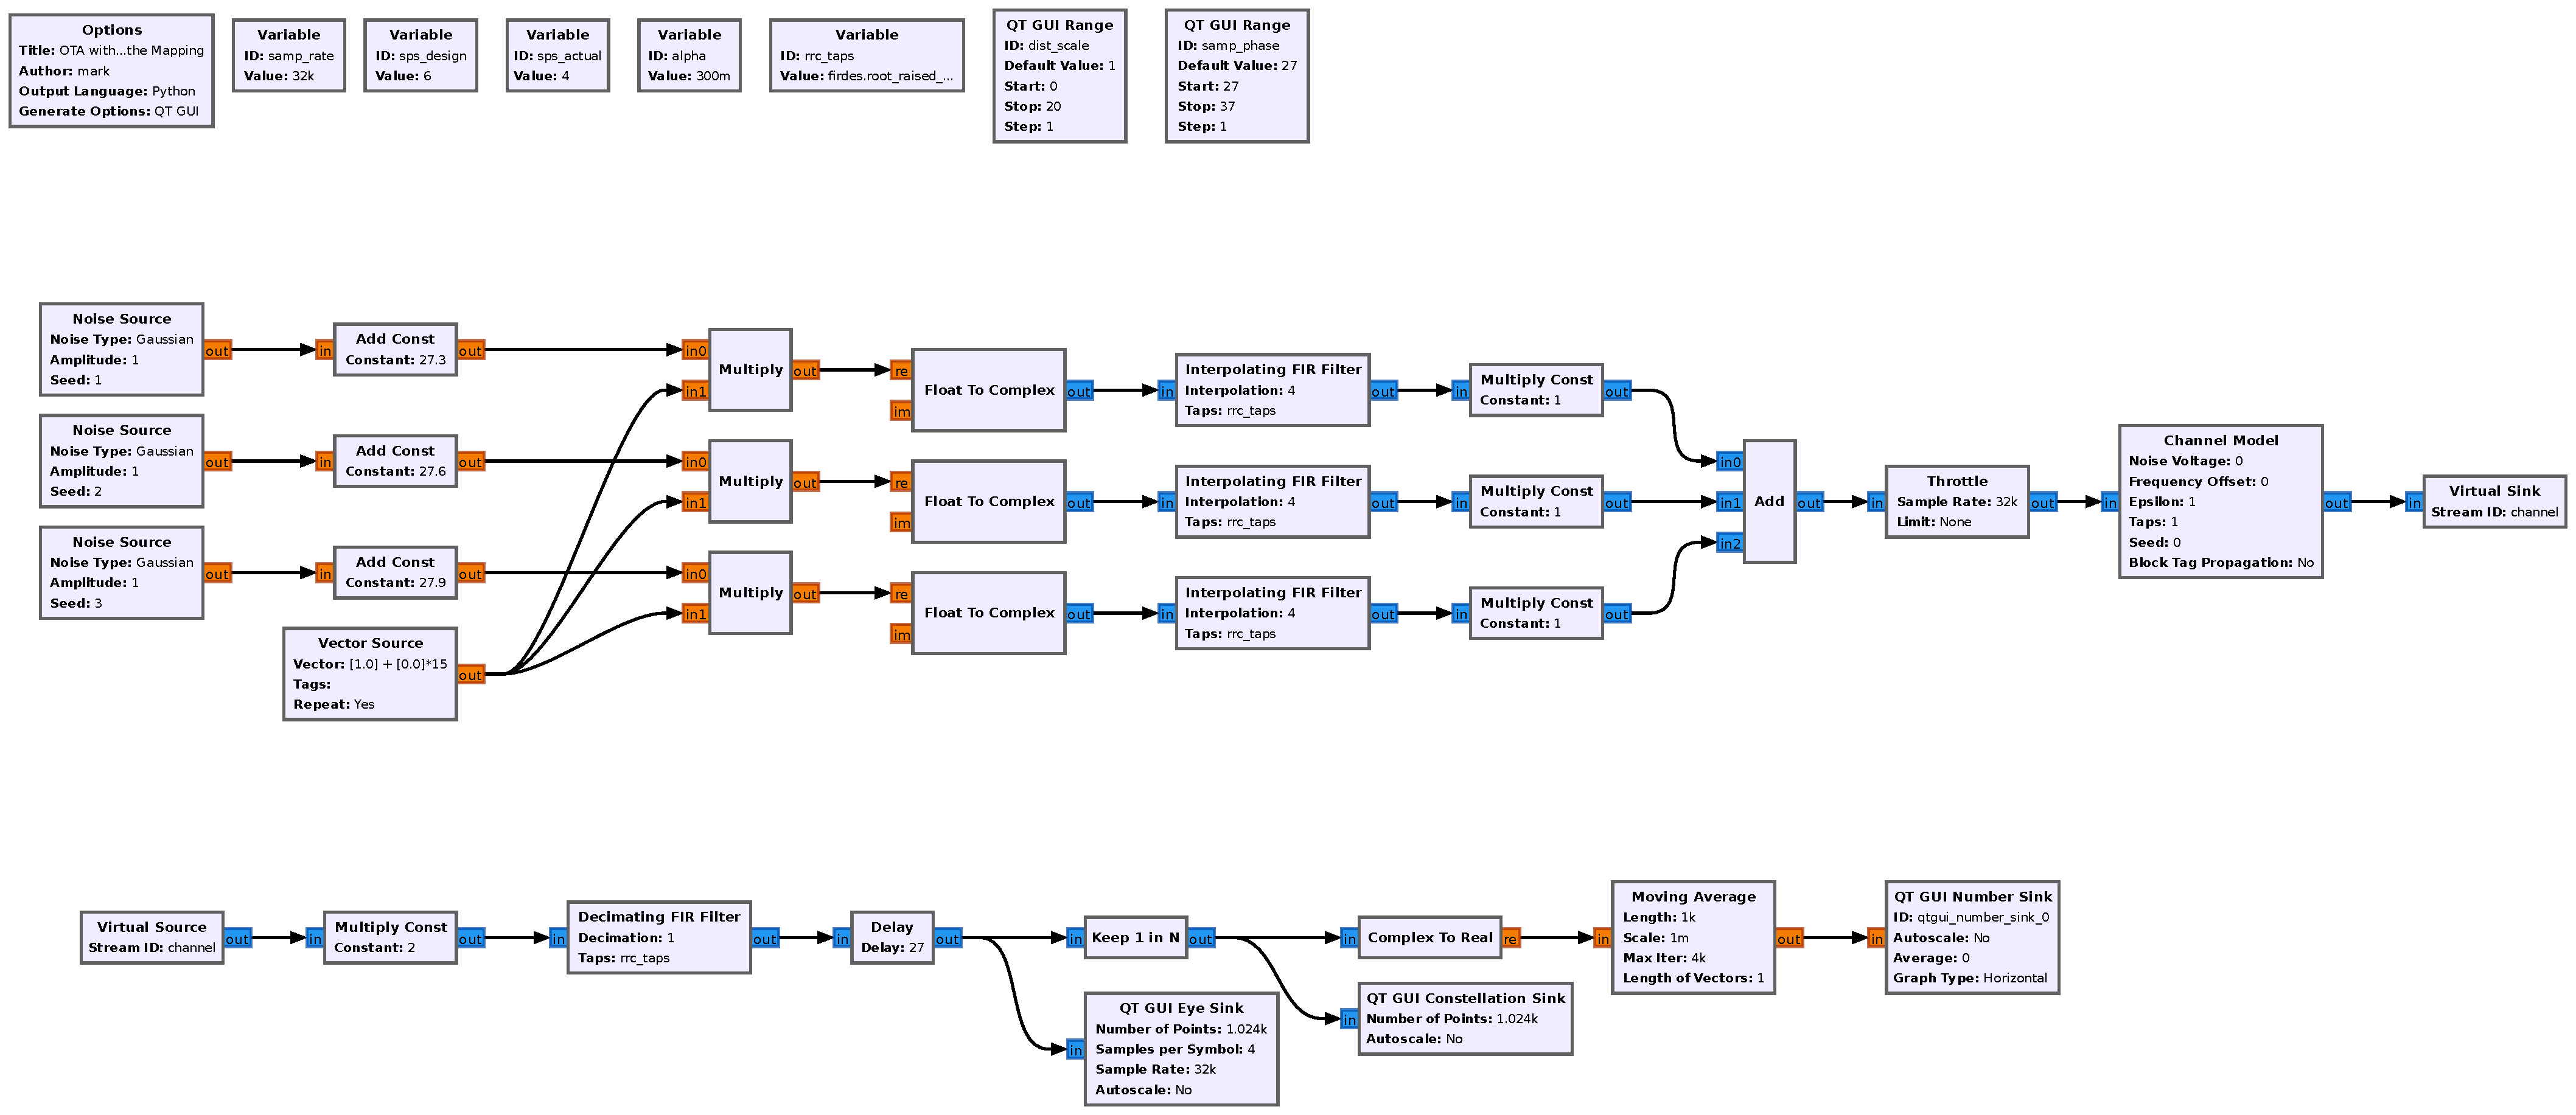
\includegraphics[width=\linewidth]{flowgraphs/OTAwithISI.pdf}
            \caption{GNU Radio Companion flowgraph for the OTA implementation including Channel Model and RRC filters.}
            \label{fig:ota_analog}
        \end{figure}
        
        \begin{figure}[htpb]
            \centering
            \includegraphics[width=\linewidth]{img/ota&isi_matched.png}
            \caption{GNU Radio Companion flowgraph configured to induce Intersymbol Interference (ISI) by mismatching the design and actual sampling rates.}
            \label{fig:ota_isi_matched}
        \end{figure}

    \subsection{MATLAB and Simulink Integration}
        While GNU Radio provides a robust framework for real-time SDR execution and analog signal evaluation, future phases of this methodology will incorporate MATLAB Simulink. Simulink will be utilized to model advanced feedback loops, custom waveform generation, and digital equalizers (e.g., Minimum Mean Square Error (MMSE) receivers) that are mathematically complex to implement in standard GNU Radio environments. This dual-software approach allows for both practical SDR validation and rigorous mathematical algorithmic design.

    \ifSubfilesClassLoaded{
        \clearpage
        \printbibliography
    }{}

\end{document}